Die Messapparatur ist wie folgt vorgegeben:
\begin{figure}[h!]
  \centering
  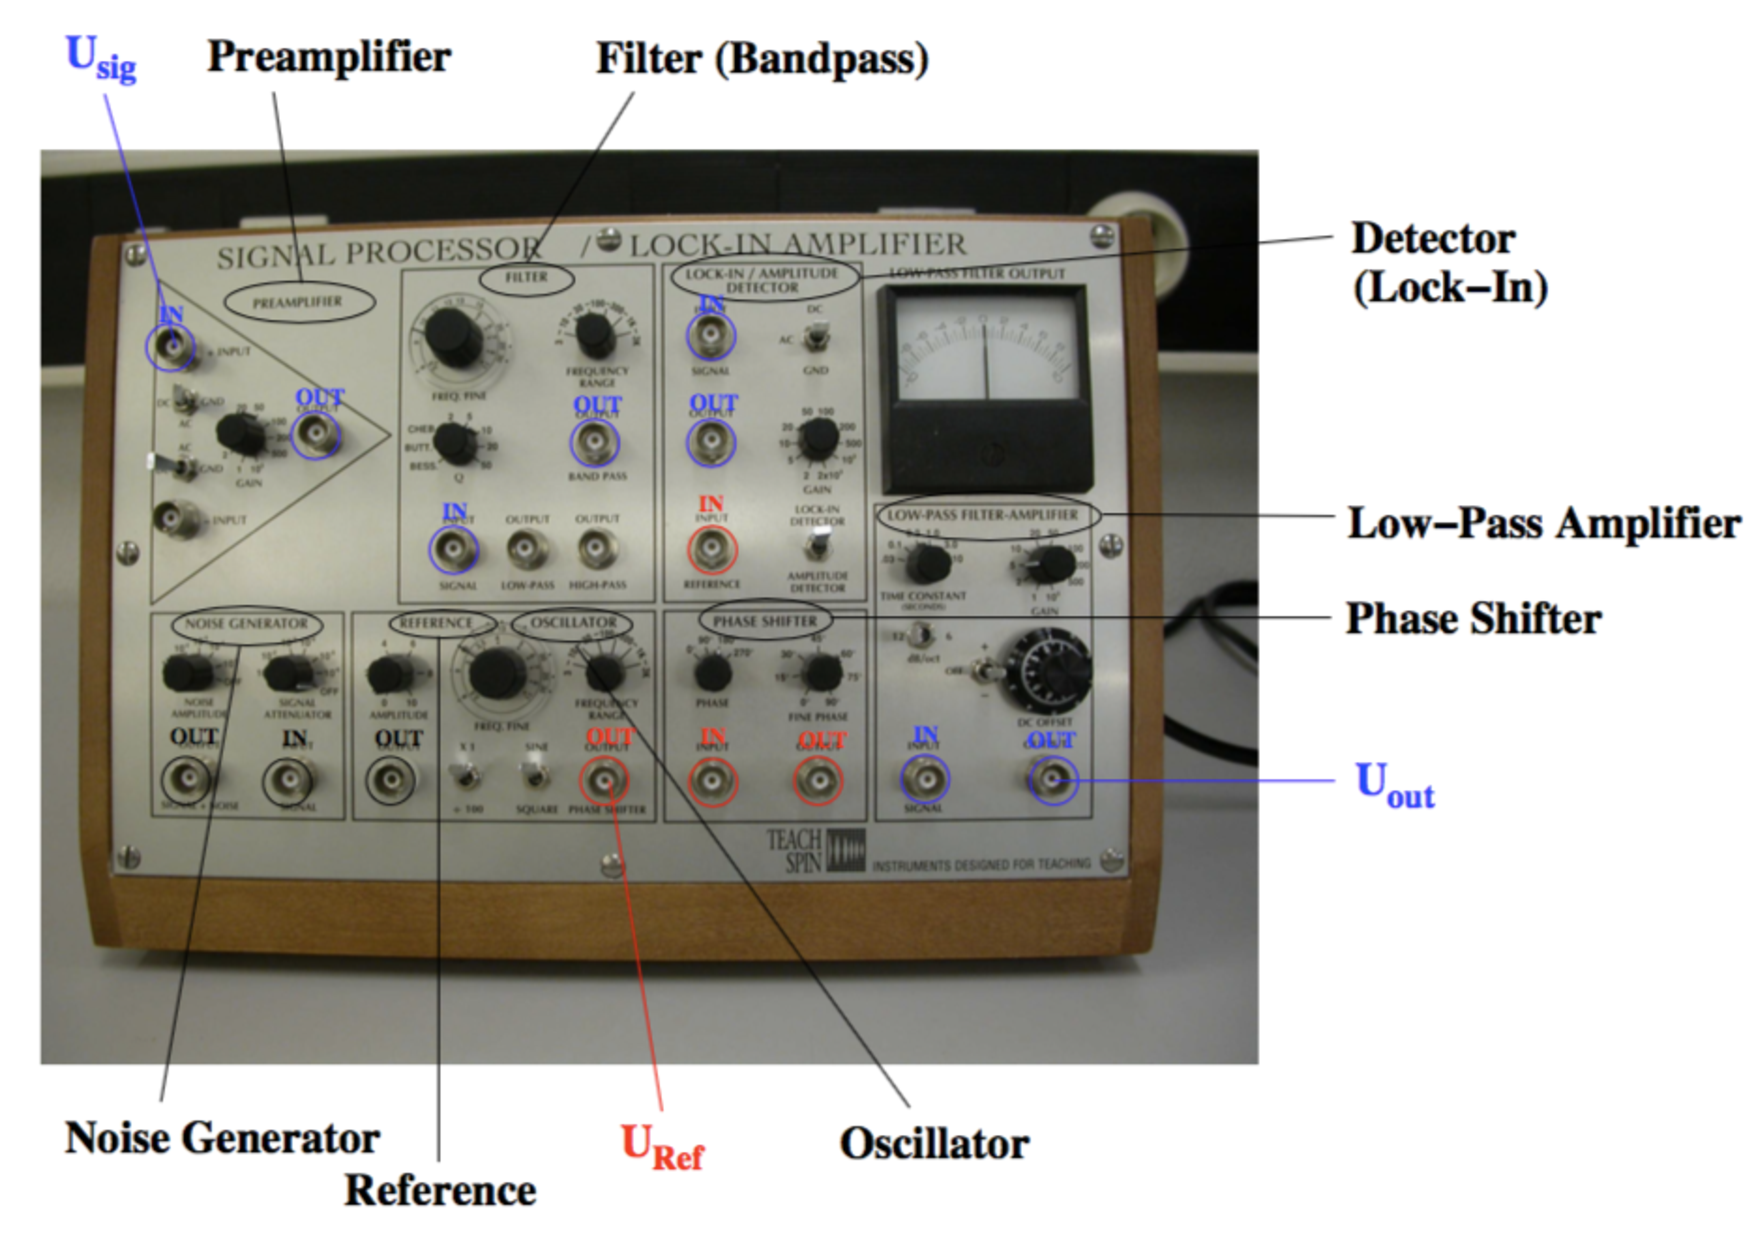
\includegraphics[width=\textwidth]{LockIn.pdf}
  \caption{Lock-In-Verstärker \cite{1}}
  \label{fig:LIV}
\end{figure}
\\Darin sind ein Vorverstärker, ein Bandpass-Filter, ein Lock-In-Detektor, ein Störgenerator, ein Funktionsgenerator, ein Phasenschieber und ein Tiefpass-Verstärker verbaut.
\\Außerdem ist ein Oszilloskop vorhanden.
\\Zunächst wird geprüft, welcher Ausgang des Funktionsgenerators eine veränderliche Amplitude generiert und welcher eine konstante Amplitude generiert.
Der Ausgang "Reference Out" liefert eine veränderliche Amplitude, der Ausgang "Oscillator Phase Out" gibt eine konstante Amplitude von $U_{0}=\SI{2.28}{V}$.
\\Zur Verifizierung der Funktionsweise des Lock-In-Verstärkers wird der Versuchsaufbau zur Schaltung in Abbildung \ref{fig:LockIn} gesteckt.
\begin{figure}[h!]
  \centering
  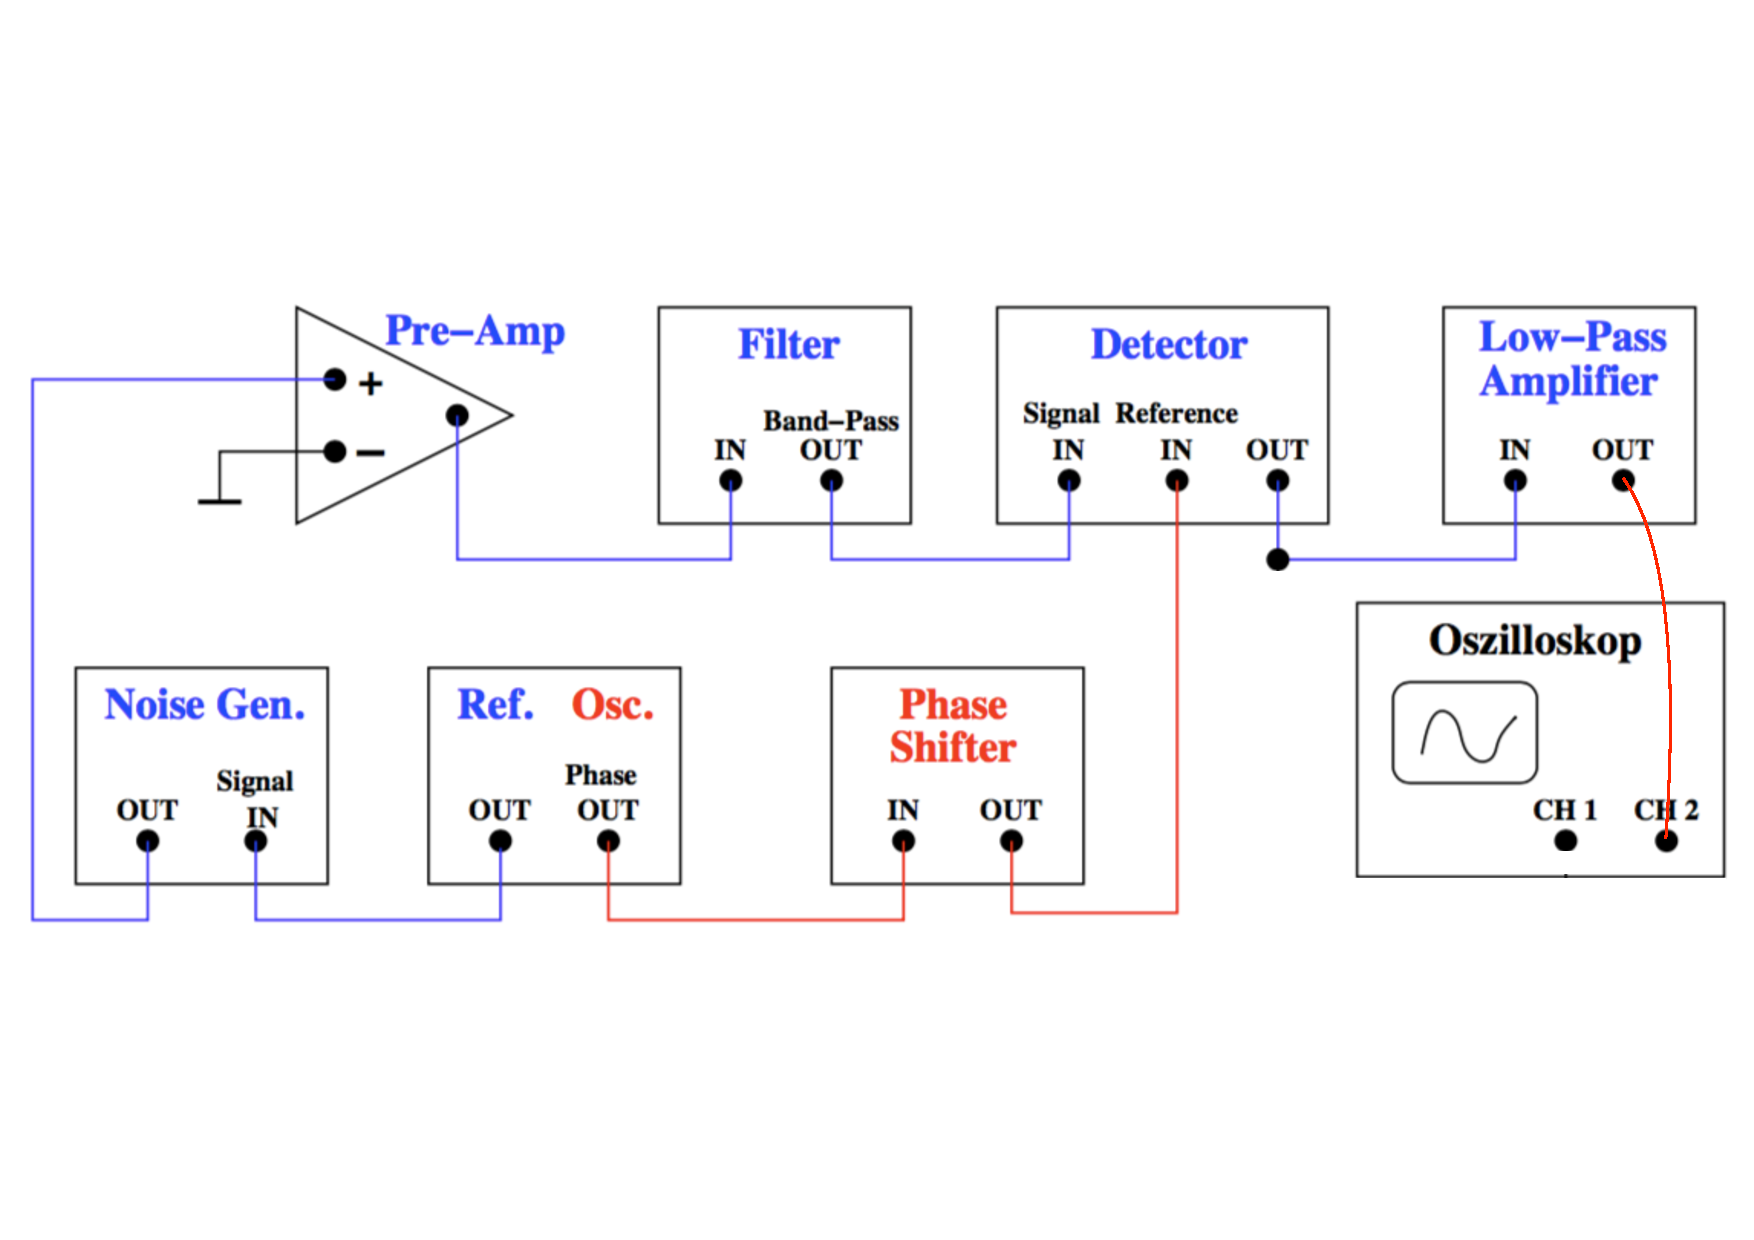
\includegraphics[width=\textwidth]{LockInSchaltung.pdf}
  \caption{Schaltung zur Verifizierung der Funktionsweise des Lock-In-Verstärkers \cite{1}}
  \label{fig:LockIn}
\end{figure}
\\Der Störgenerator wird jedoch zunächst überbrückt.
Es wird eine Sinusspannung $U_{ref}$ mit dem Funktionsgenerator generiert.
\\Die Ausgangsspannung wird für fünf verschiedene Phasenverschiebungen gespeichert.
Für zehn verschiedene Phasen wird die Amplitude gemessen und aufgetragen.
\\Der Störgenerator wird zugeschaltet.
Die weiteren Einstellungen der Schaltung werden beibehalten.
Die Amplitude wird für zehn Phasen gemessen und die Ausgangsspannungen werden für fünf Phasen gespeichert.
\\Für die Messung mit der Photodetektorschaltung wird eine Photodiode und ein Photodetektor in die Schaltung wie in Abbildung \ref{fig:Photo} eingebaut.
\begin{figure}[h!]
  \centering
  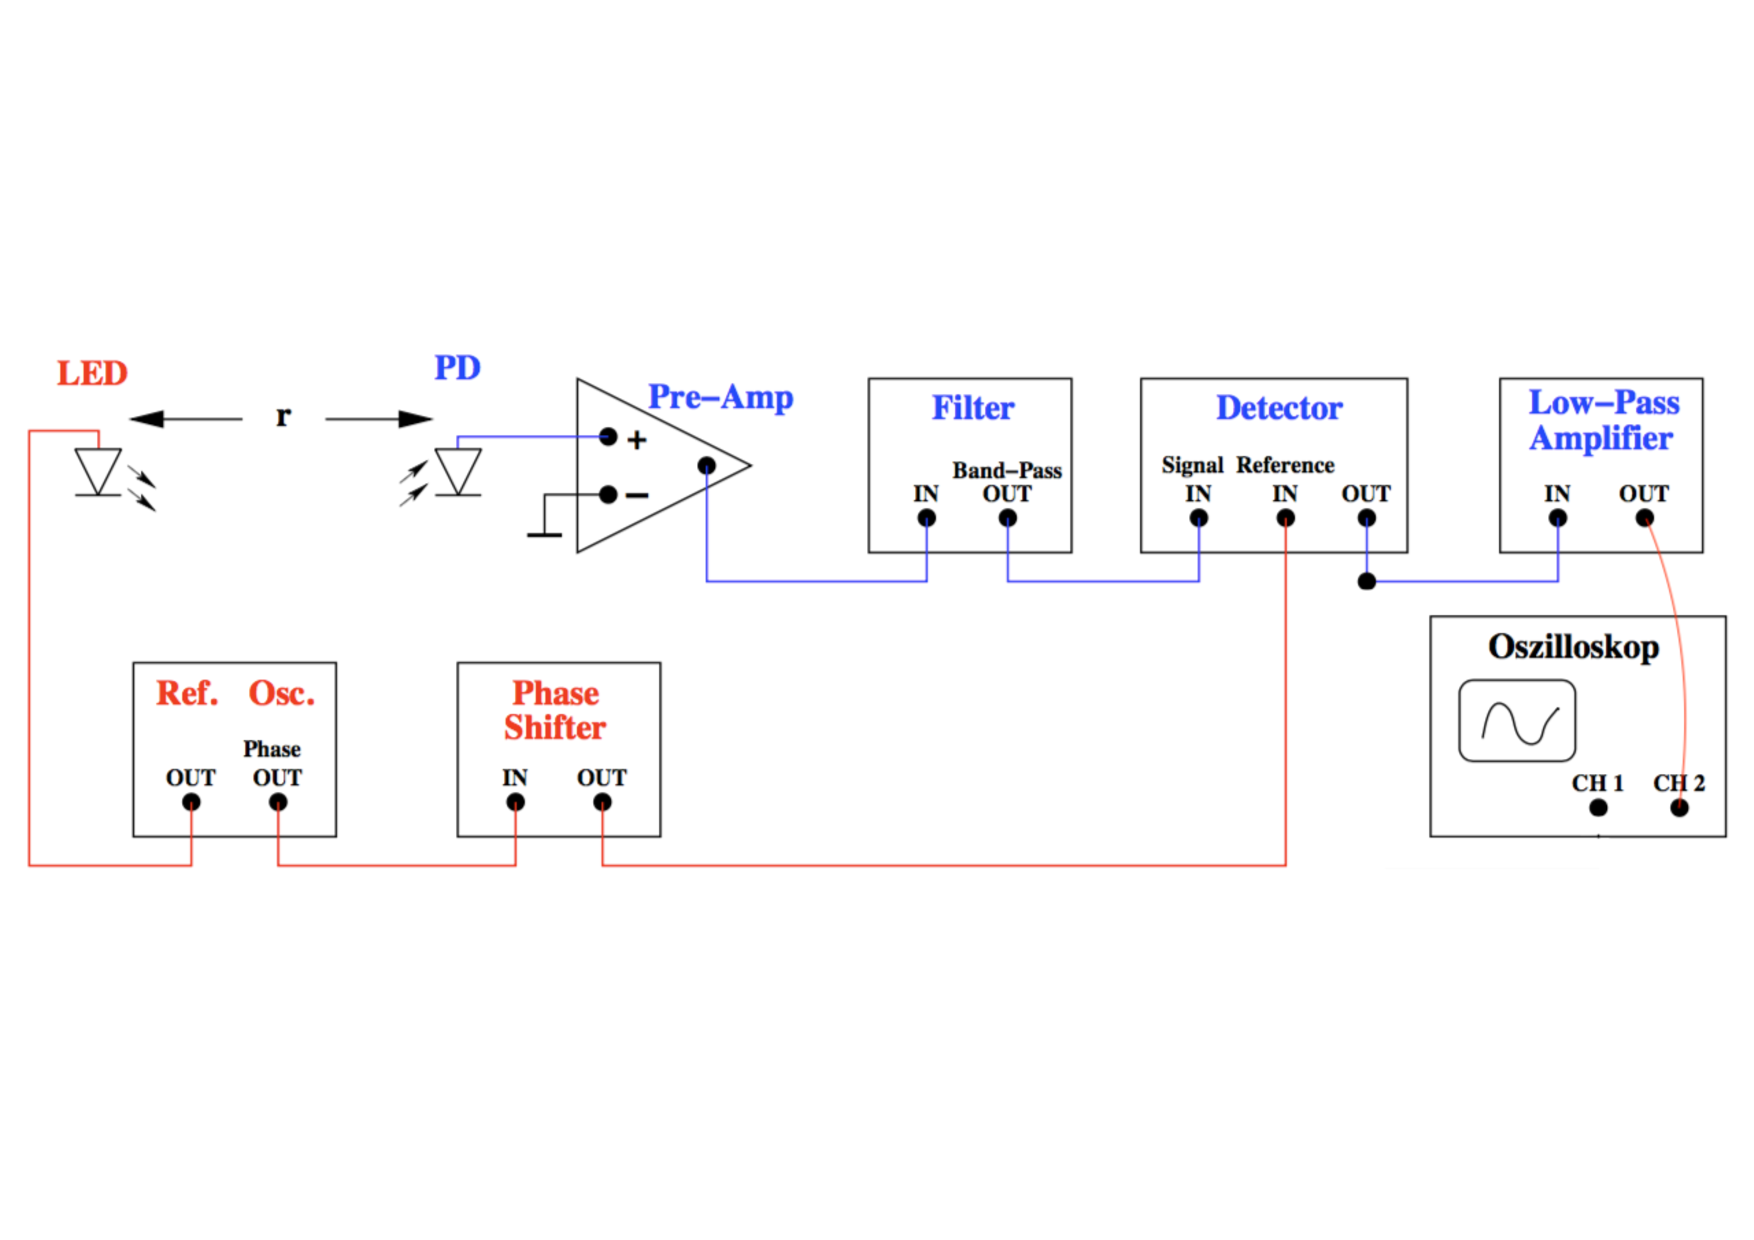
\includegraphics[width=\textwidth]{Photodetektor.pdf}
  \caption{Schaltung zur Rauschunterdrückung mit dem Photodetektor \cite{1}}
  \label{fig:Photo}
\end{figure}
\\Die Diode wird auf eine Frequenz von $f=\SI{199,6}{Hz}$ und eine Spannung von $U=2V$ eingestellt.
Die Intensität $U_{I}$ wird mit dem Abstand $x$ zur Diode gemessen.



\FloatBarrier
